\chapter{Rate Limiting And Fairness}
\textbf{Intro}
\\\\
Not all the users of \textit{Tor} wish to service as much as they can, they maybe want to limit their service and bandwidth usage. In this chapter we will investigate the Tors approach toward rate limiting and fairness.\\\\
\textbf{Tors Approach}\\
\\
Tor takes the \textit{token bucket} approach (see Fig \ref{fig:Token_bucket}) for achieving rate limiting to the users. with this approach, the average rate of output will be equal to incoming bytes while allowing short-term burst. so with this approach in practice the incoming bytes to be transferred will be limited.\\
\\
\begin{figure}[!h]
\centering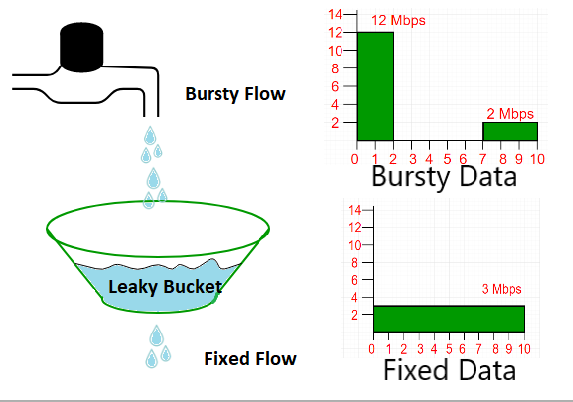
\includegraphics[scale=0.4]{token_bucket}
\caption{Token Bucket Approach - from \textit{geekforgeeks.com} website}
\label{fig:Token_bucket} % Unique label used for referencing the figure in-text
\end{figure}
\\
\\
\textbf{Distinguishing Interactive and Bulk Streams }\\
\\
have in mind that for TCP connections, for every bit of information to transfer we have to transfer a whole cell of 512 bytes (we can't wait to receive enough bytes to fill-up the cell, maybe it is an interactive scenario that the sender waits for the reply ).\\
In-order to better service the clients, Tor distinguishes between bulk streams and interactive streams by their frequency in which they supply cells. the algorithm and idea is based on Rennhard et al’s design. with this approach Tor tries to give a preferential service to interactive streams and good overall service ( best effort ) to bulk streams. but have in mind with this preferential services the timing end-to-end attack is possible.\\

\textbf{Rate Limiting Implementation}\\
\\
Tor, as we mentioned before, uses a token bucket approach ( one for reads, one for writes ).\\
Since version 0.2.0.X tor let the clients use additional token buckets to specify their strict rate limiting policies on the "relayed" traffic.\\
To avoid partitioning concerns we combine both classes of traffic over a given OR connection, and keep track of the last time we read or wrote a high-priority (non-relayed) cell. If it's been less than N seconds (currently N=30), we give the whole connection high priority, else we give the whole connection low priority. We also give low priority to reads and writes for connections that are serving directory information. see proposal 111 for more details.\\
\\




